\documentclass[a4paper]{article}
\usepackage[T1]{fontenc}			% pacchetto per \chapter
\usepackage[italian]{babel}
\usepackage[italian]{isodate}  		% formato delle date in italiano
\usepackage{graphicx}				% gestione delle immagini
\usepackage{amsfonts}
\usepackage{booktabs}				% tabelle di qualità superiore
\usepackage{amsmath}				% pacchetto matematica
\usepackage{stmaryrd} 				% per '\llbracket' e '\rrbracket'
\usepackage{amsthm}					% teoremi migliorati
\usepackage{enumitem}				% gestione delle liste
\usepackage{pifont}					% pacchetto con elenchi carini


\usepackage[x11names]{xcolor}		% pacchetto colori RGB
% Link ipertestuali per l'indice
\usepackage{xcolor}
\usepackage[linkcolor=black, citecolor=blue, urlcolor=cyan]{hyperref}
\hypersetup{
	colorlinks=true
}

%\usepackage{showframe}				% visualizzazione bordi
%\usepackage{showkeys}				% visualizzazione etichetta

\newtheorem{theorem}{Teorema}
\renewcommand{\qedsymbol}{QED}
\newcommand{\exec}[1]{\llbracket #1\:\rrbracket}
\newcommand{\dquotes}[1]{``#1''}

\begin{document}
	% indice
	\tableofcontents
	
	\newpage
	
	\section{Introduzione alla materia}
	
	Prima di iniziare con la presentazione di alcuni concetti fondamentali, si definisce l'\textbf{invariante induttiva}: pensando a qualsiasi linguaggio di programmazione, una generica condizione è \underline{sempre} vera prima, durante e dopo un ciclo. Questo concetto ritornerà in futuro.
	
	\subsection{Cardinalità degli insiemi}
	Il motivo dell'interesse di un ripasso di un argomento trattato in passato è giustificato dal fatto che i dati manipolati in informatica sono (e)numerabili, ovvero è possibile metterli in corrispondenza biunivoca con i numeri naturali, essendo essi stessi rappresentati da numeri (binari).
	
	Di seguito viene mostrato un richiamo ai concetti di base in relazione alla cardinalità di insiemi:
	\begin{itemize}
		\item[\ding{80}] \textbf{Cardinalità.} Se $S$ è un insieme, la sua \textbf{\emph{cardinalità}} si rappresenta con il simbolo $|S|$.
	
		\item[\ding{80}] \textbf{Equipotenza.} Due insiemi $A$ e $B$ sono \textbf{\emph{equipotenti}} se esiste una funzione biiettiva del tipo $f: A \rightarrow B$ (cioè una funzione sia iniettiva che suriettiva; approfondimento: \href{https://www.youmath.it/lezioni/analisi-matematica/le-funzioni-da-r-a-r-in-generale/7-iniettivita-suriettivita-e-invertibilita-di-una-funzione-generica.html}{link}, oppure qui di seguito). \newline
		La \textbf{\emph{rappresentazione}} matematica è la seguente $A \approx B$.\newline
		La relazione $|A| \le |B|$ è possibile se esiste una funzione iniettiva $f: A \rightarrow B$. Si osservi che la funzione $f$ stabilisce una corrispondenza tra gli elementi dei due insiemi. Infatti, l'\textbf{iniettività} assicura che la corrispondenza è stabilita elemento per elemento, mentre la \textbf{surriettività} assicura che la quantità degli oggetti nei due insiemi coincide.
	
		\item[\ding{80}] \textbf{Insiemi finiti e infiniti.} Negli \textbf{\emph{insiemi finiti}}, la cardinalità è un numero naturale corrispondente al numero di oggetti contenuti nell'insieme.\newline
		Invece, negli \textbf{\emph{insiemi infiniti}} la $|A|$ rappresenta la collezione degli insiemi $Y$ tale che $Y \approx A$. Questa collezione viene chiamata \textbf{cardinalità} di $A$. Quindi, è vero che se $A \subseteq B$ allora si deduce che $|A| \le |B|$.
		
		\item[\ding{80}] \textbf{Insieme numerabile.} Un insieme $A$ viene detto \textbf{\emph{numerabile}} se è finito o equipotente all'insieme dei numeri naturali $\mathbb{N}$ (ovvero, $A \approx \mathbb{N}$). \newline
		La cardinalità degli insiemi infiniti numerabili è denotata con $\mathfrak{N}_0$. \newline
		Un insieme $A$ è finito se $|A| < \mathfrak{N}_0$. Quindi, un insieme è numerabile se $|A| \le \mathfrak{N}_0$ (ovvero se è finito, quindi minore, oppure se è un insieme infinito numerabile rappresentato come $\mathfrak{N}_0$, quindi uguale).
	\end{itemize}
	
	\newpage
	
	\subsection{Alcune notazioni}
	
	Se un generico \textbf{\emph{linguaggio di programmazione}} viene indicato con la lettera $\mathfrak{L}$ e un generico \textbf{\emph{algoritmo}} di un programma viene indicato con la lettera $A$, allora se un \emph{algoritmo viene implementato in un linguaggio di programmazione}, è possibile scrivere la notazione insiemistica $A \in \mathfrak{L}$. In un linguaggio di programmazione \underline{è possibile scrivere infiniti programmi}, ovvero l'insieme dei numeri naturali $\mathbb{N}$. \newline
	\noindent
	Esistono due tipi di \textbf{\emph{rappresentazioni}}:

	\begin{itemize}
		\item[\ding{42}] \textbf{Rappresentazione intensionale.} Rappresenta solo l'algoritmo, più nello specifico solamente quella specifica parte di codice (esempio a fine elenco).
		
		\item[\ding{42}] \textbf{Rappresentazione estensionale.} Rappresenta l'insieme ma tramite una forma più estesa (esempio a fine elenco).
	\end{itemize}
	
	L'\textbf{\emph{esecuzione}} di un determinato algoritmo si indica con delle parentesi quadre più spesse $\exec{A}$. Quindi, la sua \emph{rappresentazione intensionale} è solamente $A$, mentre la sua \emph{rappresentazione estensionale} è data da $\exec{A}(i) = o$ ($i$ è input e $o$ è output). La rappresentazione estensionale può essere anche nel seguente modo $\exec{M} \in \left\{f\: | \: f =\exec{M}\right\}$
	con $f = \left\{ \left(x, f(x)\right)\: | \: x \in \mathbb{N}\right\}$.
	
	Un programma restituisce uno o più risultati come numeri naturali $\mathbb{N}$, prendendo in input dei numeri naturali $\mathbb{N}$. Quindi, più formalmente si può scrivere $\mathbb{N} \longrightarrow \mathbb{N}$. Questa rappresentazione non è altro che la definizione dei \textbf{\emph{problemi \label{def:problema}}} esistenti. Difatti, l'informatica si pone il dubbio che esista una certa soluzione ($f$), scritta sotto forma di algoritmo appartenente ad un linguaggio di programmazione, tale che la sua esecuzione dia la soluzione. Più formalmente:
	
	\begin{equation*}
		\mathbb{N} \longrightarrow \mathbb{N} \ni f \hspace{2em}
		\exists A \in \mathfrak{L} : \exec{A} = f
	\end{equation*}
	
	\newpage
	
	\subsection{Teorema di Cantor (1874)}
	
	Il seguente teorema ha come conseguenza che \textbf{esistono insiemi non numerabili}. Questo risultato si attribuisce a Georg Cantor, matematico tedesco, nel 1874.
	
	La \textbf{dimostrazione} è importante da capire. Essa utilizza una tecnica, detta dimostrazione diagonale, che è alla base di gran parte dei risultati principali che stabiliscono i fondamenti dell'informatica come scienza (Dauben, 1979; \href{https://www.cambridge.org/core/journals/journal-of-symbolic-logic/article/abs/joseph-warren-dauben-georg-cantor-his-mathematics-and-philosophy-of-the-infinite-harvard-university-press-cambridge-mass-and-london-1979-ix-404-pp/52B6E0EDBF207D9023F9526866CDF92D}{Official Cambridge article link}).
	
	\begin{theorem}[\textbf{Cantor}] \label{cantor}
		\begin{equation}
			|\mathbb{N}| < |\mathbb{N} \longrightarrow \mathbb{N}|
		\end{equation}
		La cardinalità di $\mathbb{N}$ (numero di programmi per risolvere problemi) è strettamente più piccolo della cardinalità delle funzioni $\mathbb{N} \longrightarrow \mathbb{N}$ (numero di problemi esistenti).
	\end{theorem}

	\begin{proof}[\textbf{Dimostrazione}]
		Si supponga per assurdo che $|\mathbb{N}| = |\mathbb{N}\longrightarrow\mathbb{N}|$. Questo implica che esistono funzioni numerabili come per esempio $f_0, f_1, f_2, ..., f_x, ...$.
		
		La genialità di Cantor si manifesta quando pensa ad una funzione $g(x)$ così definita:
	
		\begin{equation*}
			g(x) = f_{x}(x) + 1 \hspace{2em} \text{con } g:\mathbb{N}\longrightarrow\mathbb{N}
		\end{equation*}
	
		Con ovviamente $x\in\mathbb{N}$. La funzione $g(x)$ prende un numero naturale e restituisce un numero naturale, quindi è correttamente identificabile come un problema (definizione di problema a pagina~\pageref{def:problema}) e matematicamente formalizzabile come $\mathbb{N}\longrightarrow\mathbb{N}$.
		
		Dunque, prendendo qualsiasi funzione $f$ numerata $x$-esima, essa sarà diversa dalla funzione $g$ numerata $x$-esima poiché sempre aumentata di $1$:
		
		\begin{equation*}
			f_{x}(x) \ne g(x) \longrightarrow f_{x}(x) \ne f_{x}(x) + 1
		\end{equation*}
	\end{proof}

	Questo teorema purtroppo non è possibile applicarlo agli algoritmi informatici poiché se al posto della funzione $f_{x}(x)$ venisse inserito un algoritmo e quest'ultimo non terminasse mai, dunque sostituibile con $\infty$, la somma $+1$ non verrebbe mai eseguita. Per esempio, quando un programma entra in un loop che non gli consente di eseguire le istruzioni successive.
	
	\newpage
	
	
	
	\subsection{Problema decisionale e ipotesi del continuo}
	
	Un \textbf{\emph{alfabeto}} è una sequenza di simboli con cui è possibile scrivere gli algoritmi risolutivi. L'alfabeto utilizzato nelle realizzazioni tecnologiche è l'\textbf{alfabeto binario} $\Sigma = \{0, 1\}$.
	
	Un \textbf{\emph{problema decisionale}} è la versione associata ad un dato problema informatico $f\in\mathbb{N}\longrightarrow\mathbb{N}$, ovvero alla funzione:
	
	\begin{equation}\label{problema_decisionale}
		d_{f} : \mathbb{N}\times\mathbb{N}\longrightarrow\{0,1\}
	\end{equation}

	\noindent
	Definita nel seguente modo:
	
	\begin{equation*}
		d_{f} ((x,y)) = 
		\begin{cases}
			1 & \text{se}\:y = f(x)\\
			0 & \text{altrimenti}
		\end{cases}
	\end{equation*}
	
	\noindent
	Un problema decisionale non è altro che una funzione con co-dominio $\{0,1\}$ che è in grado di decidere se una data coppia $(x,y)\in\mathbb{N}\times\mathbb{N}$ appartiene ad $f$.
	
	Essendo un problema decisionale una funzione associata ai problemi in informatica, allora esiste la relazione:
	\begin{equation*}
		\mathbb{N}\longrightarrow\{0,1\}\subseteq\mathbb{N}\longrightarrow\mathbb{N}
	\end{equation*}
	
	\noindent
	Dunque, sicuramente sarà vera la seguente condizione:
	\begin{equation*}
		|\mathbb{N}\longrightarrow\{0,1\}| \le |\mathbb{N}\longrightarrow\mathbb{N}|
	\end{equation*}

	\noindent
	Ma sarà vera anche la seguente:
	\begin{equation*}
		|\mathbb{N}\longrightarrow\{0,1\}| = |\mathbb{N}\longrightarrow\mathbb{N}|
	\end{equation*}

	\begin{proof}[\textbf{Dimostrazione}]
		È chiaro che la seguente relazione è vera:
		\begin{equation*}
			|\mathbb{N} \times \mathbb{N}| = |\mathbb{N}|
		\end{equation*}
	
		\noindent
		Allora, vale anche:
		\begin{equation*}
			|\mathbb{N}\longrightarrow\{0,1\}| = |\mathbb{N}\times\mathbb{N}\longrightarrow\{0,1\}|
		\end{equation*}
		
		\noindent
		Si prenda qualsiasi funzione del tipo $f: \mathbb{N} \longrightarrow \mathbb{N}$. A tale funzione, viene associato l'insieme:
		\begin{equation*}
			S_{f} = \left\{
			(i, o)\: | \: f(i) = o
			\right\} \subseteq \mathbb{N} \times \mathbb{N}
		\end{equation*}
		
		\noindent
		In cui $i$ indica l'input e $o$ indica l'output. Viene scritta la sua relativa equazione caratteristica:
		\begin{equation*}
			f_{S_{f}} (x,y) =
			\begin{cases}
				1 & \text{se } (x,y) \in S_{f} \\
				0 & \text{altrimenti}
			\end{cases}
		\end{equation*}
	
		\noindent
		Allora si può affermare con certezza:
		\begin{equation}\label{uguaglianza_problema_decisionale}
			|\mathbb{N}| < |\mathbb{N} \longrightarrow \mathbb{N}| = |\mathbb{N} \longrightarrow \{0,1\}| = |2^{\mathbb{N}}| = |\mathbb{R}|
		\end{equation}
	
		\noindent
		L'ultima uguaglianza è possibile grazie all'\textbf{ipotesi del continuo}.
	\end{proof}

	\newpage
	
	
	
	
	\section{Linguaggi regolari ed automi a stati finiti}
	
	\subsection{Alfabeti e Linguaggi}
	
	Qui di seguito si lasciano una serie di definizioni utili per il futuro:
	
	\begin{itemize}
		\item[\ding{42}] \textcolor{Red3}{\textbf{\emph{Simbolo.}}} \textbf{Entità primitiva astratta} che non viene definita formalmente (come punto, linea, etc.).\newline
		\underline{Per esempio}, lettere e caratteri numerici sono simboli.
		
		\item[\ding{42}] \textcolor{Red3}{\textbf{\emph{Alfabeto.}}} Rappresentato con la lettera greca Sigma $\Sigma$, è un \textbf{insieme finito di simboli}.
		
		\item[\ding{42}] \textcolor{Red3}{\textbf{\emph{Stringa (o parola).}}} \textbf{Sequenza finita di simboli giustapposti}, ovvero messi uno affianco all'altro.\newline
		\underline{Per esempio}, se $a$, $b$, $c$ sono simboli, allora $abcba$ è una stringa.
		
		\item[\ding{42}] \textcolor{Red3}{\textbf{\emph{Lunghezza di una stringa.}}} Viene denotata con $|w|$, in cui $w$ è una stringa, e rappresenta il \textbf{numero di occorrenze di simboli che compongono una stringa}. \underline{Ad esempio}, $|abcba| = 5$.\newline
		Attenzione che la \textcolor{Red3}{\textbf{stringa vuota}} viene denotata con $\varepsilon$ ed è la \textbf{stringa costituita da zero simboli}: $|\varepsilon| = 0$.
		
		\item[\ding{42}] \textcolor{Red3}{\textbf{\emph{Concatenazione di stringhe.}}} Due stringhe $v$ e $w$ sono concatenate quando si rappresentano nel seguente modo $vw$. Si \textbf{ottiene facendo seguire alla prima stringa la seconda}.\newline
		La concatenazione è un'\textbf{operazione} che ammette come identità la stringa vuota $\varepsilon$.
		
		\item[\ding{42}] \textcolor{Red3}{\textbf{\emph{Linguaggio formale.}}} Detto anche linguaggio $L$, è un \textbf{insieme di stringhe di simboli da un alfabeto} $\Sigma$. L'insieme vuoto $\emptyset$ e l'insieme $\{\varepsilon\}$ sono due linguaggi formali di qualunque alfabeto. L'insieme $\emptyset$ \textbf{non contiene elementi}, mentre l'insieme $\{\varepsilon\}$ \textbf{ne contiene uno}, ovvero la stringa vuota $\longrightarrow$ \underline{sono insiemi diversi!}
		
		\item[\ding{42}] \textcolor{Red3}{\textbf{\emph{Sequenze finite.}}} Rappresentate con $\Sigma^*$, è il \textbf{linguaggio costituito da tutte le stringhe su un fissato alfabeto} $\Sigma$. Quindi, viene considerato anche il \textbf{linguaggio più grande esistente}, ovvero il limite superiore. Tuttavia, questo non implica che sia il linguaggio più efficiente o potente (argomento approfondito in futuro). In parole povere, è l'insieme delle sequenze di stringhe \underline{finite}.\newline
		\underline{Definizione matematica:}

		\begin{equation*}
			\Sigma^* = \left\{a_1 \cdots a_n \: | \: n \ge 0, a_i \in \Sigma\right\}
		\end{equation*}
	\end{itemize}
	
	\noindent
	Sia quindi $L \subseteq \Sigma^*$ un \textbf{generico linguaggio formale} sull'alfabeto $\Sigma$.
	
	\newpage
	
	\subsection{Operazioni sui linguaggi}
	
	Sia $\Sigma$ un alfabeto e $L$, $L_1$, $L_2$ insiemi di stringhe di $\Sigma^*$. Le \textbf{operazioni sui linguaggi} sono principalmente tre:
	
	\begin{itemize}
		\item[\ding{45}] \textcolor{Red3}{\textbf{\emph{Concatenazione.}}} La \textbf{concatenazione} di $L_1$ e $L_2$, denotata con $L_1 \cdot L_2$ è l'insieme:
		
		\begin{equation*}
			L_{1}L_{2} = \left\{xy \in \Sigma^{*} \: | \: x \in L_1, y \in L_2 \right\}
		\end{equation*}
	
		Si definisce dunque:
	
		\begin{equation*}
			\begin{cases}
				L^{0} = \left\{\varepsilon\right\} \\
				L^{n+1} = L \cdot L^{n}
			\end{cases}
		\end{equation*}
		
		E facendo attenzione al fatto $L^{0} = \left\{\varepsilon\right\} \ne \emptyset$.
	
		\item[\ding{45}] \textcolor{Red3}{\textbf{\emph{Complemento.}}} Il \textbf{complemento} di un linguaggio è denotato con $\bar{L}$:
		
		\begin{equation*}
			\bar{L} = \left\{\sigma \: | \: \sigma \in \Sigma^*, \sigma \notin L\right\}
		\end{equation*}
	
		\item[\ding{45}] \textcolor{Red3}{\textbf{\emph{Chiusura di Kleene.}}} Viene denotata con $L^{*}$ ed è l'insieme così definito:
		
		\begin{equation*}
			L^{*} = \bigcup_{n \ge 0} L^n
		\end{equation*}
	
		\item[\ding{45}] \textcolor{Red3}{\textbf{\emph{Chiusura positiva.}}} Denotata con $L^{+}$ è l'insieme così definito:
		
		\begin{equation*}
			L^{+} = \bigcup_{n \ge 1} L^n
		\end{equation*}
	
		E si verifica immediatamente che $L^{+} = LL^{*}$. Quindi, questo operato si può derivare dalla chiusura e dalla concatenazione.
		
		\item[\ding{45}] \textcolor{Red3}{\textbf{\emph{Unione.}}} L'\textbf{unione} tra due linguaggi, che corrisponde ad un \textbf{\emph{or logico}}, è così definita:
		
		\begin{equation*}
			L_{1} \cup L_{2} = \left\{\sigma \: | \: \sigma \in L_{1} \lor \sigma \in L_{2} \right\}
		\end{equation*}
	
		\item[\ding{45}] \textcolor{Red3}{\textbf{\emph{Intersezione.}}} L'\textbf{intersezione} tra due linguaggi, che corrisponde ad un \textbf{\emph{and logico}}, è così definita:
		
		\begin{equation*}
			L_{1} \cap L_{2} = \left\{\sigma \: | \: \sigma \in L_{1} \land \sigma \in L_{2} \right\}
		\end{equation*}
	\end{itemize}

	\newpage
	
	\begin{center}
		\large \textcolor{Green4}{\textbf{Esempio di esercizio su linguaggi e alfabeti}}
	\end{center}

	\noindent
	Dati i seguenti dati:
	
	\begin{gather*}
		\textbf{Alfabeto: } \Sigma = \left\{a, b\right\} \\
		\textbf{Linguaggio: } L = \left\{a, b\right\}
	\end{gather*}

	\noindent
	Si costruisce l'insieme $L^{*}$, ovvero il linguaggio costituito da tutte le stringhe su un fissato alfabeto. Per definizione uguale anche a $\Sigma^{*}$:
	
	\begin{equation*}
		L^{*} = \left\{\varepsilon, a, b, aa, ab, ba, bb, \cdots\right\} = \Sigma^{*}
	\end{equation*}

	\noindent
	In cui la prima lettera, ovvero $\varepsilon$, può essere rappresentato con $L^{0}$;\newline
	Le lettere $\left\{a\right\}$ e $\left\{b\right\}$, insieme a $L^{0}$, possono essere rappresentate con $L^{1}$; \newline
	Le lettere $\left\{aa\right\}$, $\left\{ab\right\}$, $\left\{ba\right\}$, $\left\{bb\right\}$, insieme a $L^0$ e $L^{1}$, possono essere rappresentate con $L^{2}$;\newline
	E così via. Date che sono infinite stringhe componibili, il linguaggio viene associato a $\Sigma^{*}$.
	
	\newpage
	
	\subsection{Automa a stati finiti}
	
	Un \textbf{automa a stati finiti} è un \underline{modello matematico} di un sistema avente un input ed eventualmente un output, a valori discreti. Il sistema può essere in uno stato tra un insieme finito di stati possibili. Essendo in uno stato, l'automa ha la possibilità di \textbf{tenere traccia della storia precedente}.
	
	\noindent
	Analizzando letteralmente le parole di ``automa a stati finiti'':
	
	\begin{itemize}
		\item[\ding{46}] \textbf{\emph{Automa.}} Macchine che lavorano indipendentemente dall'intervento dell'essere umano.
		
		\item[\ding{46}] \textbf{\emph{A stati finiti.}} Con \textbf{stato} si intende lo stato effettivo della macchina. Mentre con \textbf{finiti} si intende che lo stato al tempo $t$ è effettivamente finito, ovvero è una quantità di informazione finita.
	\end{itemize}
	
	Solitamente, viene rappresentato con una testina che legge da un nastro, quest'ultimo contenente la sequenza di simboli dell'alfabeto dati in input all'automa. La testina che legge si sposta sempre nella stessa direzione, consumando la sequenza in input. La testina si può trovare in un certo \textbf{\emph{stato}}; a seconda dello stato $q$ e del simbolo $s_i$ letto, la testina si porta in un certo altro stato (o rimane nello stesso) e si sposta a destra per apprestarsi a leggere il simbolo successivo dalla sequenza.
	
	\begin{figure}[!htp]
		\centering
		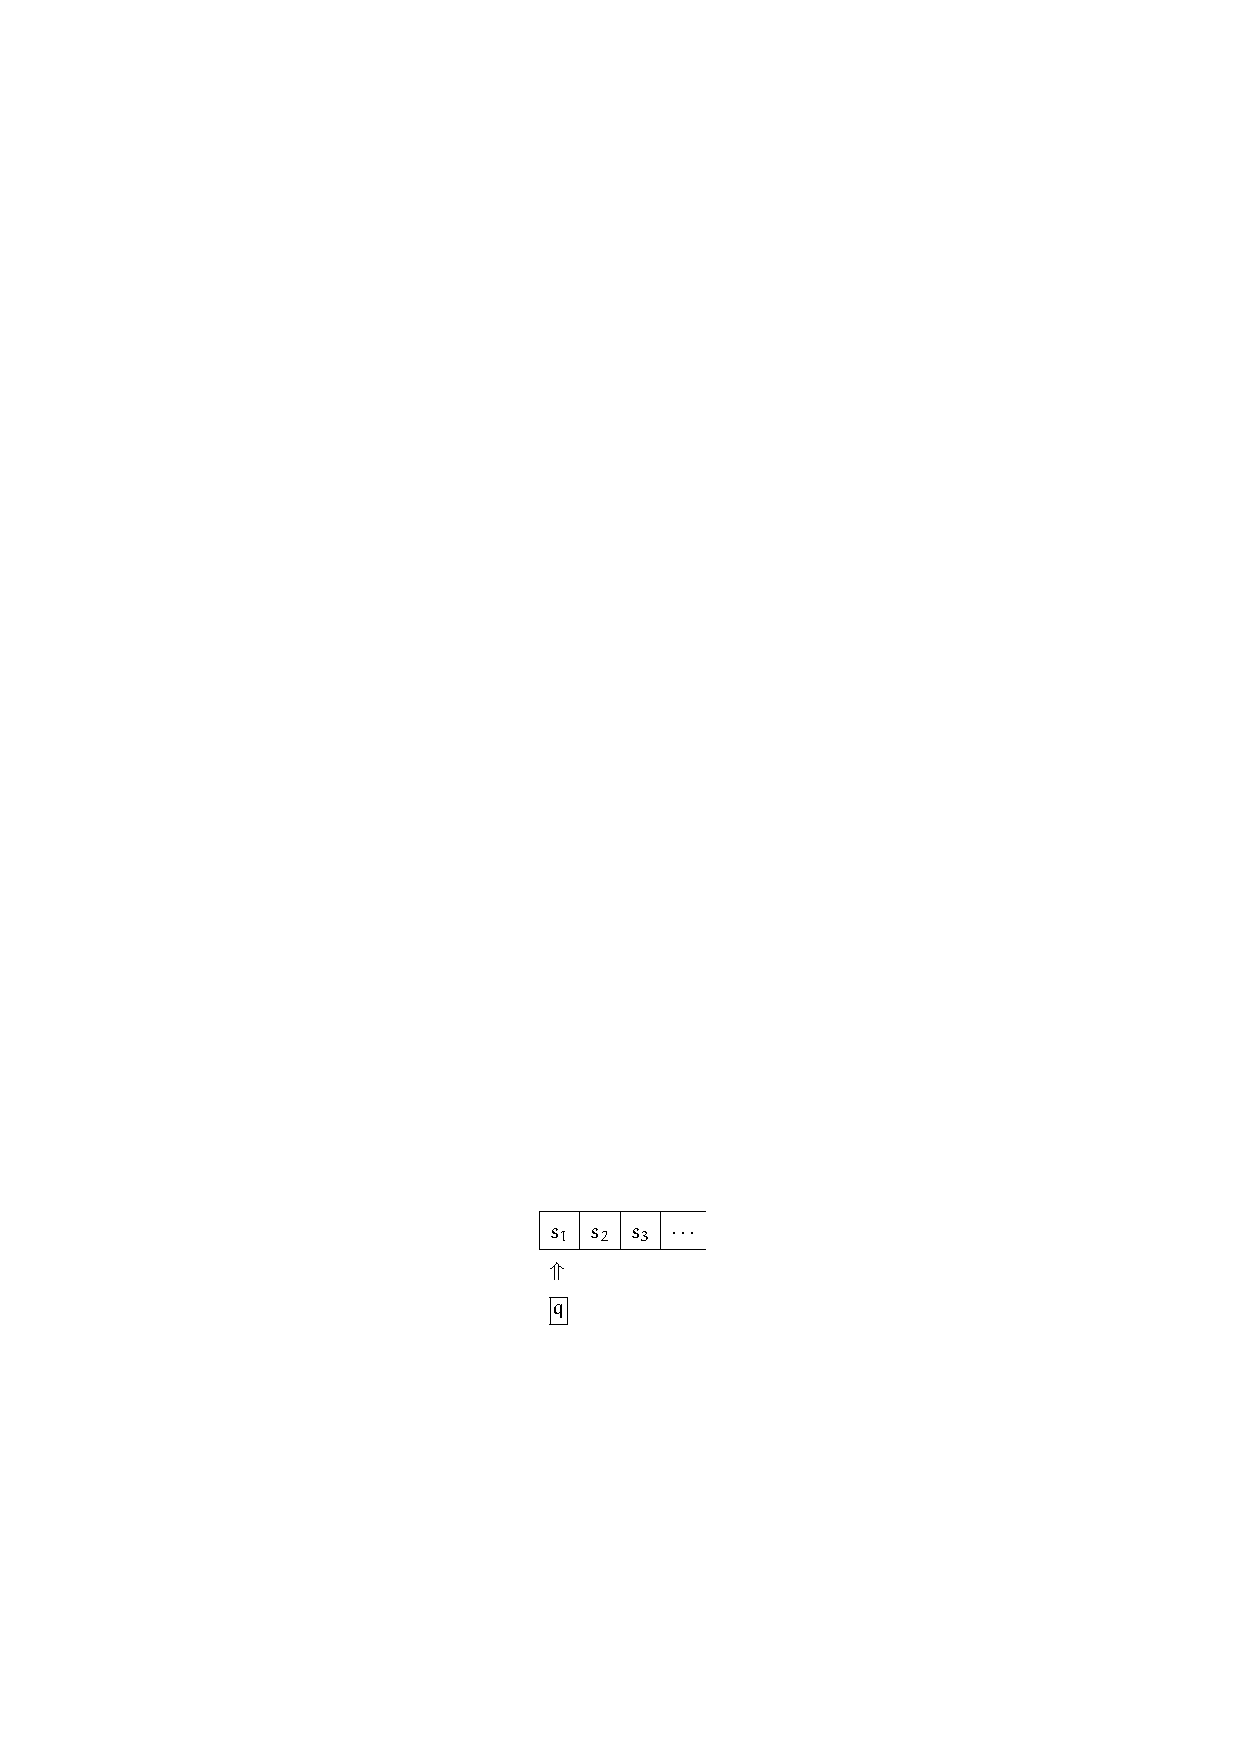
\includegraphics[width=0.3\textwidth]{img/automa_generale.pdf}
		\caption{Dispositivo che rappresenta un esempio generalistico di un automa a stati finiti.}
	\end{figure}

	Una volta terminata la lettura, l'automa è in grado di fornire il risultato di accettazione o di refutazione della stringa (parola) letta. Il \textbf{comportamento} dell'automa si \textbf{definisce} in maniera univoca mediante una tabella, chiamata \textbf{matrice di transizione}, come ad esempio:
	
	\begin{table}[!htbp]
		\centering
		
		\begin{tabular}{@{} c c c @{}}
			\toprule
			 & $a$ & $b$ \\
			\midrule
			$q_{0}$ & $q_{1}$ & $q_{2}$ \\
			$q_{1}$ & $q_{1}$ & $q_{0}$ \\
			$q_{2}$ & $q_{1}$ & $q_{0}$ \\
			\bottomrule
		\end{tabular}
		
		\caption{Matrice di transizione.}
		\label{matrice_di_transizione}
	\end{table}

	\newpage

	\noindent
	Tuttavia, la \underline{rappresentazione più comune e chiara} è il \textbf{grafo}:
	
	\begin{itemize}
		\item Gli \textbf{archi} rappresentano le \emph{transizioni} etichettate con il simbolo in lettura;
		\item Lo \textbf{stato iniziale} è rappresentato con la \emph{freccia ``start''};
		\item Gli \textbf{stati finali} sono cerchiati due volte.
	\end{itemize}

	\begin{figure}[!htp]
		\centering
		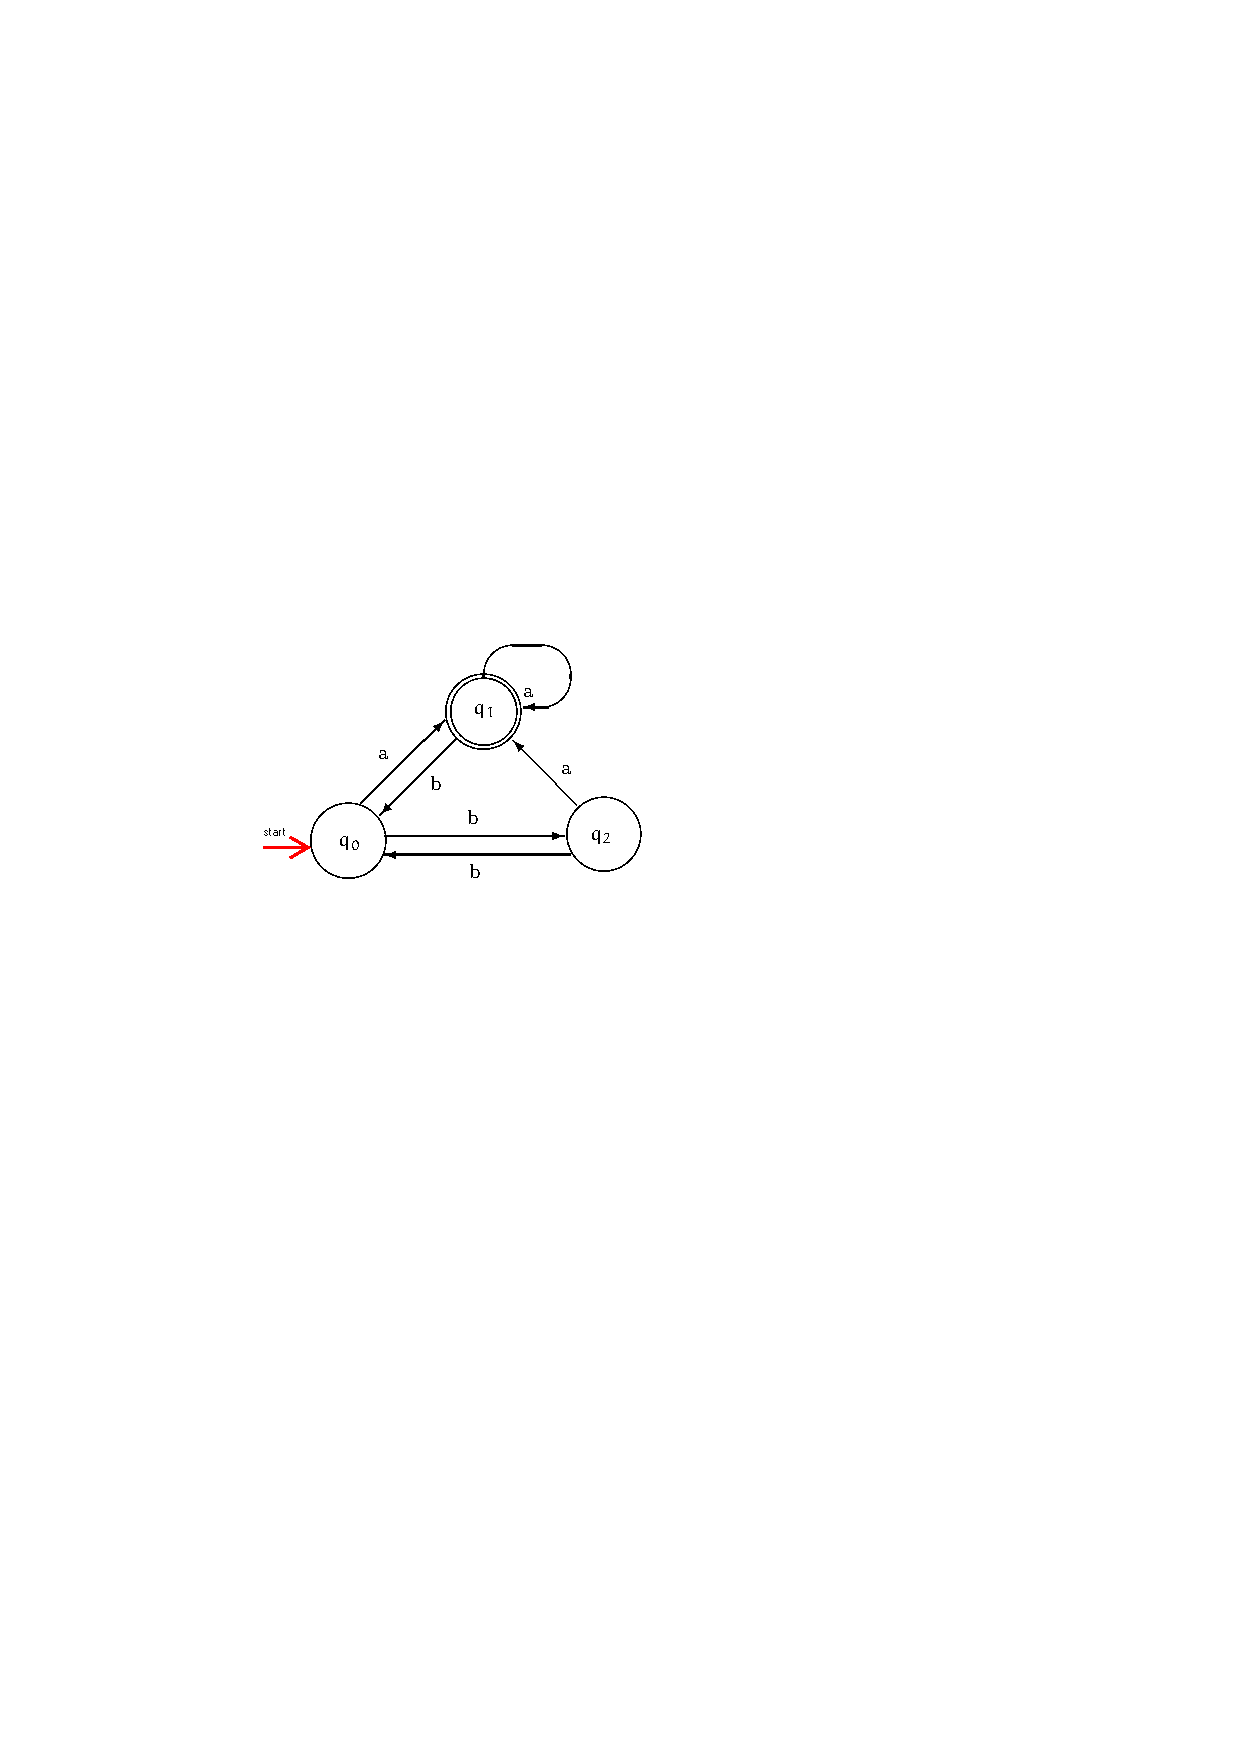
\includegraphics[width=0.5\textwidth]{img/grafo_eg.pdf}
		\caption{Esempio di grafo (freccia start mancante).}
	\end{figure}

	Un \textcolor{Red3}{\textbf{linguaggio vuoto}} è il più piccolo dei linguaggi, si rappresenta con il simbolo $\emptyset$ e si riconosce poiché \textbf{non ha stati finiti} (quindi nessun nodo con il doppio cerchio). Infine, il \textcolor{Red3}{\textbf{linguaggio più grande}} è il linguaggio più grande, si rappresenta con il simbolo $\Sigma^{*}$, esiste dunque la relazione $\emptyset \subseteq \Sigma^{*}$ e si riconosce perché \textbf{ha \underline{solo} stati finiti} (quindi nessun nodo con un solo cerchio).

	\newpage

	\subsubsection{Automi deterministici (DFA)}\label{automi deterministici}
	
	Un \textbf{automa a stati finiti \underline{deterministico}} (DFA) è una che, date determinate condizioni, è possibile determinare la serie di operazioni. Viene rappresentato con una quintupla del tipo $\left\langle Q, \Sigma, \delta, q_0, F\right\rangle$ in cui:
	
	\begin{itemize}
		\item[\ding{42}] $Q$ è un insieme di \textcolor{Red3}{\textbf{stati finiti}};
		
		\item[\ding{42}] $\Sigma$ è un \textcolor{Red3}{\textbf{alfabeto finito}}, cioè un alfabeto di input;
		
		\item[\ding{42}] $\delta: Q \times \Sigma \longrightarrow Q$ è la \textcolor{Red3}{\textbf{funzione di transizione}} che dato lo stato $q \in Q$ in cui si trova la macchina ed un simbolo $a \in \Sigma$ in lettura del nastro, produce il prossimo stato $\delta (q,a) \in Q$ in cui si troverà la macchina;
		
		\item[\ding{42}] $q_0$ è lo \textcolor{Red3}{\textbf{stato iniziale}};
		
		\item[\ding{42}] $F \subseteq Q$ è l'insieme degli \textcolor{Red3}{\textbf{stati finali}}, anche detti \textbf{di accettazione}.
		
		\item[\ding{42}] $\overset{\wedge}{\delta}: Q \times \Sigma^{*} \longrightarrow Q$ si ottiene dalla funzione $\delta$ ed è definita nel seguente modo:
		
		\begin{equation*}
			\begin{cases}
				\overset{\wedge}{\delta}(q, \varepsilon) = q \\
				\overset{\wedge}{\delta}(q, wa) = \delta \left(\overset{\wedge}{\delta}(q, w), a\right)
			\end{cases}
		\end{equation*}
	\end{itemize}

	Sia $M = \left\langle Q, \Sigma, \delta, q_0, F\right\rangle$ un automa a stati finiti \underline{deterministico}. Una \textbf{stringa} $x$ è detta \textbf{accettata} da un $M$ se $\overset{\wedge}{\delta}(q_{0}, x) \in F$. Inoltre, il \textbf{linguaggio è accettato dalla macchina} $M$, denotato come $L(M)$, è l'insieme di tutte le stringhe accettate da $M$, ovvero:
	
	\begin{equation*}
		L(M) = \left\{x \in \Sigma^{*} \: | \: \overset{\wedge}{\delta}(q_0, x) \in F\right\}
	\end{equation*}

	\noindent
	\textbf{N.B. A lezione al posto di $w$ e $x$ è stato utilizzato $\sigma.$}\newline
	
	\noindent
	Un linguaggio $L$ viene detto \textcolor{Red3}{\textbf{\emph{linguaggio regolare}}} se è accettato da qualche automa a stati finiti deterministico (DFA), ovvero se esiste $M$ tale che $L = L(M)$.
	
	\newpage
	
	\subsubsection{Esempio esercizio (automi deterministici)}
	
	\textcolor{Red3}{\textbf{\emph{Esercizio.}}}
	
	\noindent
	Il grafo dell'esercizio è il seguente:
	
	\begin{figure}[!htp]
		\centering
		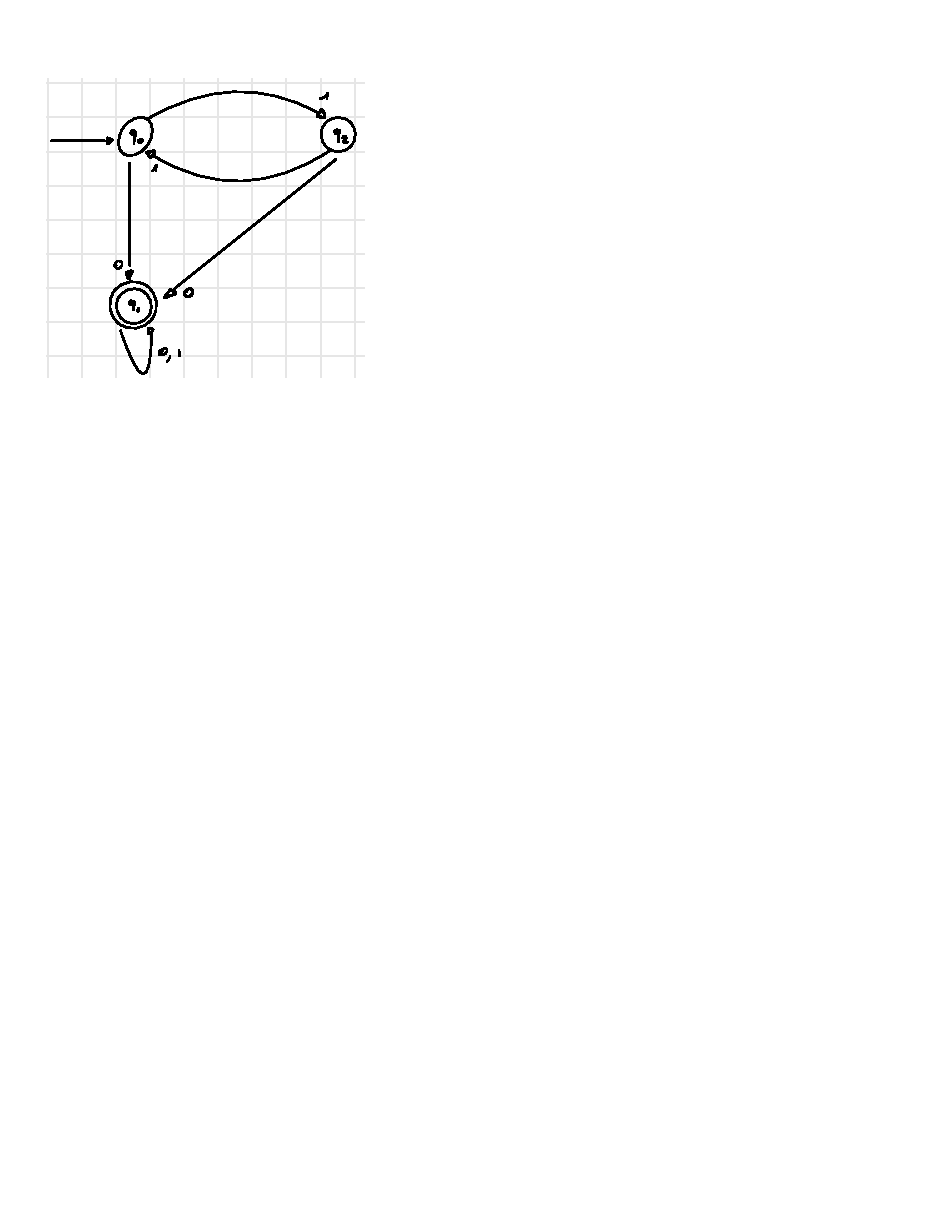
\includegraphics[width=0.6\textwidth]{img/grafo_ex1.pdf}
		\caption{Grafo di un automa a stati finiti deterministico.}
	\end{figure}
	
	\noindent
	I dati forniti sono i seguenti:
	
	\begin{gather*}
		\textbf{Linguaggio: } L(M) = \left\{x \in \{0, 1\}^* \: | \: x \text{ contiene almeno uno } 0 \right\} \\
		\textbf{Alfabeto: } \Sigma = \left\{0, 1\right\}
	\end{gather*}
	
	\noindent
	Si dimostri che $L(M)$ è $\subseteq$ e $\supseteq$ del linguaggio che è stato dato. Quindi, è necessario verificare le condizioni con:
	
	\begin{equation*}
		\left\{x \in \{0, 1\}^* \: | \: x \text{ contiene almeno uno } 0 \right\}
	\end{equation*}
	\newline
	\noindent
	\textcolor{Green4}{\textbf{\emph{Risoluzione.}}}
	
	\noindent
	La stringa $x$ è sicuramente formata da:
	
	\begin{equation*}
		x = 1^{n}\: 0 \: w \in \{0,1\}^{*} \text{ e } n \in \mathbb{N}
	\end{equation*}
	
	\noindent
	In cui ci deve essere un numero $n$ di concatenazioni di numeri $1$, uno $0$ come viene specificato \dquotes{$x \text{ contiene almeno uno } 0$} e infine una qualsiasi stringa dell'alfabeto $w$. L'\textbf{obbiettivo} è dimostrare che:
	
	\begin{equation*}
		\forall w \in \left\{0, 1\right\}^{*} : \overset{\wedge}{\delta} (q_{1}, w) = q_{1}
	\end{equation*}

	\noindent
	Ovvero che dato qualsiasi simbolo appartenente all'alfabeto, lo stato successivo sia sempre $q_{1}$, ovvero quello finale!
	
	\newpage
	
	Si supponga che la cardinalità di $w$, ovvero la lunghezza della stringa, sia uguale a $m$, cioè $|w| = m$. Questo implica che lo stato non varia:
	
	\begin{equation*}
		m = 0 \Longrightarrow w = \varepsilon \hspace{1em} \text{ e quindi } \hspace{1em} \overset{\wedge}{\delta} (q_{1}, w) = q_{1}
	\end{equation*}

	\noindent
	Invece, il caso in cui la stringa non sia vuota:
	
	\begin{equation*}
		m \ge 0 \text { e } m+1 \Longrightarrow w = \sigma 0 \hspace{1em} \textbf{ oppure } \hspace{1em} w = \sigma 1
	\end{equation*}

	\noindent
	Per \textbf{induzione} si riesce a dimostrare che:
	
	\begin{equation*}
		\overset{\wedge}{\delta} \left(q_{1}, \sigma 0\right) = \delta\left(\overset{\wedge}{\delta} \left(q_{1}, \sigma\right), 0\right) = \delta \left(q_{1}, 0\right) = q_{1}
	\end{equation*}
	
	\noindent
	Grazie all'induzione è stato dimostrato che se era vero per $m$, allora è vero anche per $m+1$, quindi qualsiasi $m$ (maggiore o uguale a zero ovviamente). Quindi, il \textbf{primo passo dell'esercizio è stato concluso, ovvero quello di dimostrare che la $w$ è sempre accettata soltanto se posta dopo il primo zero} (sequenza conclusiva dell'automa a stati finiti deterministico).\newline
	
	Adesso si prosegue la dimostrazione dimostrando che per ogni numero naturale, con una sequenza di $1$ si finisce nello stato $q_{0}$ o $q_{2}$, ovvero l'automa non termina.
	
	
	\noindent
	\textbf{\emph{\underline{Caso base}}}:
	
	
	\begin{itemize}
		\item $n = 0: \hspace{1em} \overset{\wedge}{\delta} \left(q_{0}, \varepsilon\right) = q_{0} \in \left\{q_{0}, q_{2}\right\}$
		\item $n \ge 0: \hspace{1em} \overset{\wedge}{\delta} \left(q_{0}, 1^{n+1}\right) = \overset{\wedge}{\delta} \left(q_{0}, 1^{n} \: 1\right) = \delta \left(\overset{\wedge}{\delta} \left(q_{0}, 1^{n}\right)\right) \in \left\{q_{0}, q_{2}\right\}$
	\end{itemize}

	\noindent
	\textcolor{Green4}{\textbf{\checkmark Dimostrato}} che ogni stringa in forma $x \in L$ (ogni stringa nel linguaggio), è accettata dall'automa. Ovvero $L \subseteq L\left(M\right)$.\newline
	
	L'esercizio si conclude con la dimostrazione $L \supseteq L\left(M\right)$- Quindi se $x$ non contiene almeno uno zero ($x = 1^{n}$), allora si può affermare con certezza che $x$ non è in $L\left(M\right) = \left\{\sigma \: | \: \overset{\wedge}{\delta} \left(q_{0}, \sigma\right) = q_{1}\right\}$. Quindi formalmente:
	
	\begin{equation*}
		\forall n : 1^{n} \Longrightarrow \overset{\wedge}{\delta} \left(q_{0}, x\right) \in \left\{q_{0}, q_{2}\right\} \hspace{2em} \textcolor{Green4}{\textbf{\checkmark Dimostrato}}
	\end{equation*}

	\newpage
	
	\subsubsection{Automi non-deterministici (NFA)}\label{automi non-deterministici}
	
	Un \textbf{automa a stati finiti \underline{non-deterministico}} (NFA) è una quintupla $\left\langle Q, \Sigma, \delta, q_0, F\right\rangle$ dove $Q, \Sigma, q_{0}$ e $F \subseteq Q$ mantengono il significato visto per gli automi deterministici (pagina~\pageref{automi deterministici}), mentre la \textbf{funzione di transizione} $\delta$ è definita come:
	
	\begin{equation*}
		\delta : Q \times \Sigma \longrightarrow P(Q) = 2^{Q} = 2^{|Q|}
	\end{equation*}

	\noindent
	Ovvero è una relazione tra stati.

	In particolare, si tratta di un concetto fondamentale in informatica che definisce un \textbf{modello (ideale)} di calcolo parallelo su cui si fonda la moderna analisi della complessità degli algoritmi.
	
	Adesso è possibile avere $\delta \left(q, a\right) = \emptyset$ per qualche $q \in Q$ ed $a \in \Sigma$, poiché l'\textcolor{Red3}{\textbf{automa non può avere transizioni per alcuni simboli in input}}.\newline
	
	\noindent
	Si definisce la funzione $\overset{\wedge}{\delta} : Q \times \Sigma^{*} \longrightarrow P\left(Q\right)$ nel seguente modo:
	
	\begin{equation*}
		\begin{cases}
			\overset{\wedge}{\delta} \left(q, \varepsilon\right) = \left\{q\right\} \\
			\overset{\wedge}{\delta} \left(q, wa\right) = \bigcup_{p \in \overset{\wedge}{\delta} \left(q, w\right)} \delta \left(p, a\right)
		\end{cases}
	\end{equation*}

	\noindent
	Inoltre, si dice che \textcolor{Red3}{\textbf{una \underline{stringa} $x$ è accettata da un automa a stati finiti non-deterministici NFA}} $M = \left\langle Q, \Sigma, \delta, q_{0}, F\right\rangle$ \textbf{se}:
	
	\begin{equation*}
		\overset{\wedge}{\delta} \left(q_{0}, x\right) \cap F \ne \emptyset
	\end{equation*}

	\noindent
	In altre parole, una stringa è accettata quando una di queste computazioni raggiunge uno stato finale dopo aver consumato la sequenza in input.

	Invece, si dice che \textcolor{Red3}{\textbf{un \underline{linguaggio} è accettato da un automa a stati finiti non-deterministici NFA}} $M$ \textbf{se corrisponde all'insieme delle stringhe accettate}:
	
	\begin{equation*}
		L\left(M\right) = \left\{x \in \Sigma^{*} \: | \: \overset{\wedge}{\delta} \left(q_{0}, x\right) \cap F \ne \emptyset\right\}
	\end{equation*}

	La rappresentazione a grafo rimane pressoché immutata. L'\textbf{unica differenza} è che da un nodo possono uscire più archi (o nessuno) etichettati dallo stesso simbolo.
	
	\newpage
	
	\subsubsection{Teorema Rabin-Scott (1959)}
	
	\begin{theorem}[\textbf{Rabin-Scott}] \label{rabin-scott}
		Sia $M = \left\langle Q, \Sigma, \delta, q_{0}, F \right\rangle$ un automa a stati finiti non deterministica (NFA). Allora esiste un automa a stati finiti deterministica $M^{'}$ tale che $L\left(M\right) = L(M^{'})$.
	\end{theorem}

	\begin{proof}[\textbf{Dimostrazione}]
		Si definisce l'automa a stati finiti non deterministica con la quintupla $M^{'} = \left\langle\ Q^{'}, \Sigma^{'}, \delta^{'}, q_{0}^{'}, F^{'} \right\rangle$ e con le seguenti proprietà:
		
		\begin{itemize}
			\item[\ding{72}] $\Sigma^{'} = \Sigma$.
			
			\item[\ding{72}] $Q^{'} = P(Q)$, sarebbe più preciso definire $Q^{'} = \left\{q_{1}, \cdots, q_{2\: |Q|}\right\}$ e poi stabilire una corrispondenza biunivoca fra tali stati e gli elementi di $P(Q)$. Tuttavia, così facendo rimane più chiara la dimostrazione.
			
			\item[\ding{72}] $q_{0}^{'} = \left\{q_{0}\right\}$.
			
			\item[\ding{72}] $F^{'} = \left\{P \subseteq Q \: | \: P \cap F \ne \emptyset\right\}$
			
			\item[\ding{72}] $\delta^{'}\left(\mathrm{P}, a\right) = \bigcup_{p \in \mathrm{P}} \delta \left(p, a\right)$, per ogni $\mathrm{P} \in P(Q)$
		\end{itemize}
	
		Si mostra, \textbf{per induzione}, sulla lunghezza della stringa di input $\sigma \in \Sigma^{*}$ che:
		
		\begin{equation}\label{induzione rabin-scott}
			\forall \sigma \in \Sigma^{*} : \overset{\wedge}{\delta} \left(q_{0}, x\right) = \overset{\wedge}{\delta^{'}} \left(q_{0}^{'}, x\right)
		\end{equation}
	
		\noindent
		In cui la parte di sinistra è per gli automi non deterministici ($\overset{\wedge}{\delta} \left(q_{0}, x\right)$), mentre la parte di destra è per gli automi deterministici $\left(\overset{\wedge}{\delta^{'}} \left(q_{0}^{'}, x\right)\right)$.\newline
		
		\noindent
		\textbf{\emph{\underline{Caso base.}}}\footnote{Il simbolo $\iff$ indica \dquotes{se e solo se}.}
		
		\begin{equation*}
			|\sigma| = 0 \iff \sigma = \varepsilon : \overset{\wedge}{\delta} \left(q_{0}, \varepsilon\right) = \left\{q_{0}\right\} = q^{'}_{0} = \overset{\wedge}{\delta^{'}} \left(q_{0}^{'}, \varepsilon\right)
		\end{equation*}
	
		\noindent
		\textbf{\emph{\underline{Passo induttivo.}}}
		
		\begin{equation*}
			\forall \sigma \in \Sigma^{*} : |\sigma| \le n : \overset{\wedge}{\delta} \left(q_{0}, \sigma\right) = \overset{\wedge}{\delta} \left(q_{0}, \sigma\right)
		\end{equation*}
	
		\noindent
		Quindi che non ci siano gli apici $'$ come nell'equazione~\ref{induzione rabin-scott}. Si dimostra induttivamente:
		
		\begin{equation*}
			\overset{\wedge}{\delta^{'}} \left(q_{0}^{'}, \sigma a\right) = \delta^{'} \left(\overset{\wedge}{\delta^{'}}\left(q_{0}^{'}, a\right), a\right) = \delta^{'} \left(\overset{\wedge}{\delta}\left(q_{0}, \sigma\right), a\right) = \bigcup_{p \in \overset{\wedge}{\delta}\left(q_{0}, \sigma\right)} \delta\left(p, a\right) = \overset{\wedge}{\delta} \left(q_{0}, \sigma a\right)
		\end{equation*}
	
		\noindent
		In cui $p \in \overset{\wedge}{\delta}\left(q_{0}, \sigma\right)$ e $\overset{\wedge}{\delta} \left(q_{0}, \sigma a\right)$ sono \textbf{macchine deterministiche}.
		
		\noindent
		La dimostrazione si conclude con le seguenti ovvie relazioni:
		
		\begin{gather*}
			\sigma \in L \iff
			\overset{\wedge}{\delta}\left(q_{0}, \sigma\right) \cap F \ne 0 \iff
			\overset{\wedge}{\delta^{'}}\left(q_{0}^{'}, \sigma\right) \cap F \ne \emptyset \iff
			\overset{\wedge}{\delta^{'}}\left(q_{0}^{'}, \sigma\right) \in F^{'} \iff
			\sigma \in L\left(M^{'}\right)
		\end{gather*}
	\end{proof}
	
	\newpage
	
	\subsubsection{Esempio esercizio (automi non-deterministici)}
	
	\textcolor{Red3}{\textbf{\emph{Esercizio.}}}
	
	\noindent
	Il grafo dell'esercizio è il seguente:
	
	\begin{figure}[!htp]
		\centering
		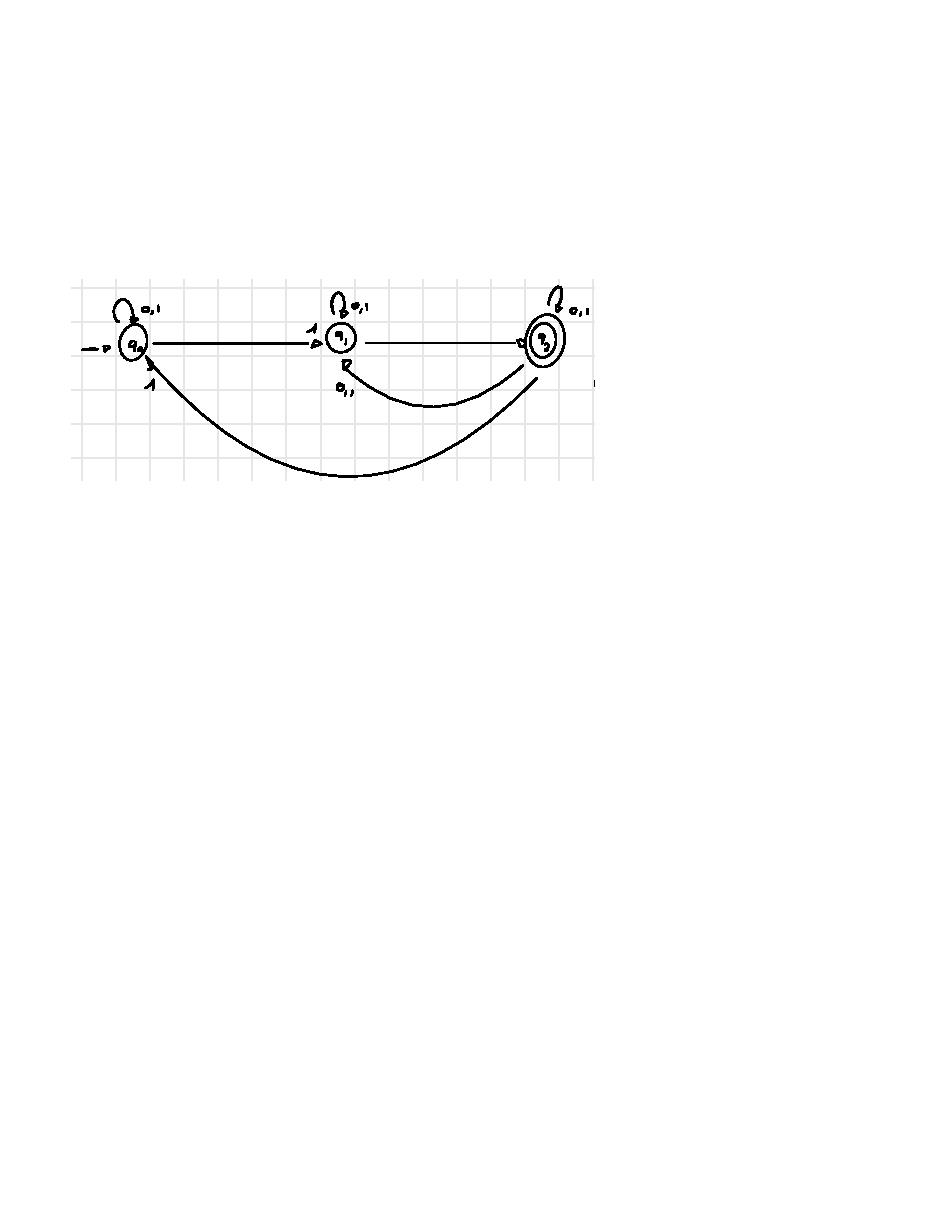
\includegraphics[width=0.7\textwidth]{img/grafo_ex2.pdf}
		\caption{Grafo di un automa a stati finiti non-deterministico.}
	\end{figure}
	
	\noindent
	\textcolor{Green4}{\textbf{\emph{Risoluzione.}}}
	
	\noindent
	La $Q$ è formata da $\left\{q_{0}, q_{1}, q_{2}\right\}$, mentre la $P(a)$ ha i seguenti insiemi:
	
	\begin{equation*}
		P\left(a\right) = \left\{
		\emptyset, \left\{q_{0}\right\},
		\left\{q_{1}\right\},
		\textcolor{Red3}{\left\{q_{2}\right\}}, \left\{q_{0}, q_{1}\right\},
		\textcolor{Red3}{\left\{q_{0}, q_{2}\right\}, \left\{q_{1}, q_{2}\right\},
		\left\{q_{0}, q_{1}, q_{2}\right\}}\right\}
	\end{equation*}

	\noindent
	Le espressioni in rosso sono sequenze finite che terminano.
	
	\noindent
	Infine, l'automa non-deterministico è riconducibile a un automa deterministico:
	
	\begin{equation*}
		\delta^{'} \left(s, a\right) = \bigcup_{q \in S} \delta \left(q, a\right)
	\end{equation*}

	\begin{figure}[!htp]
		\centering
		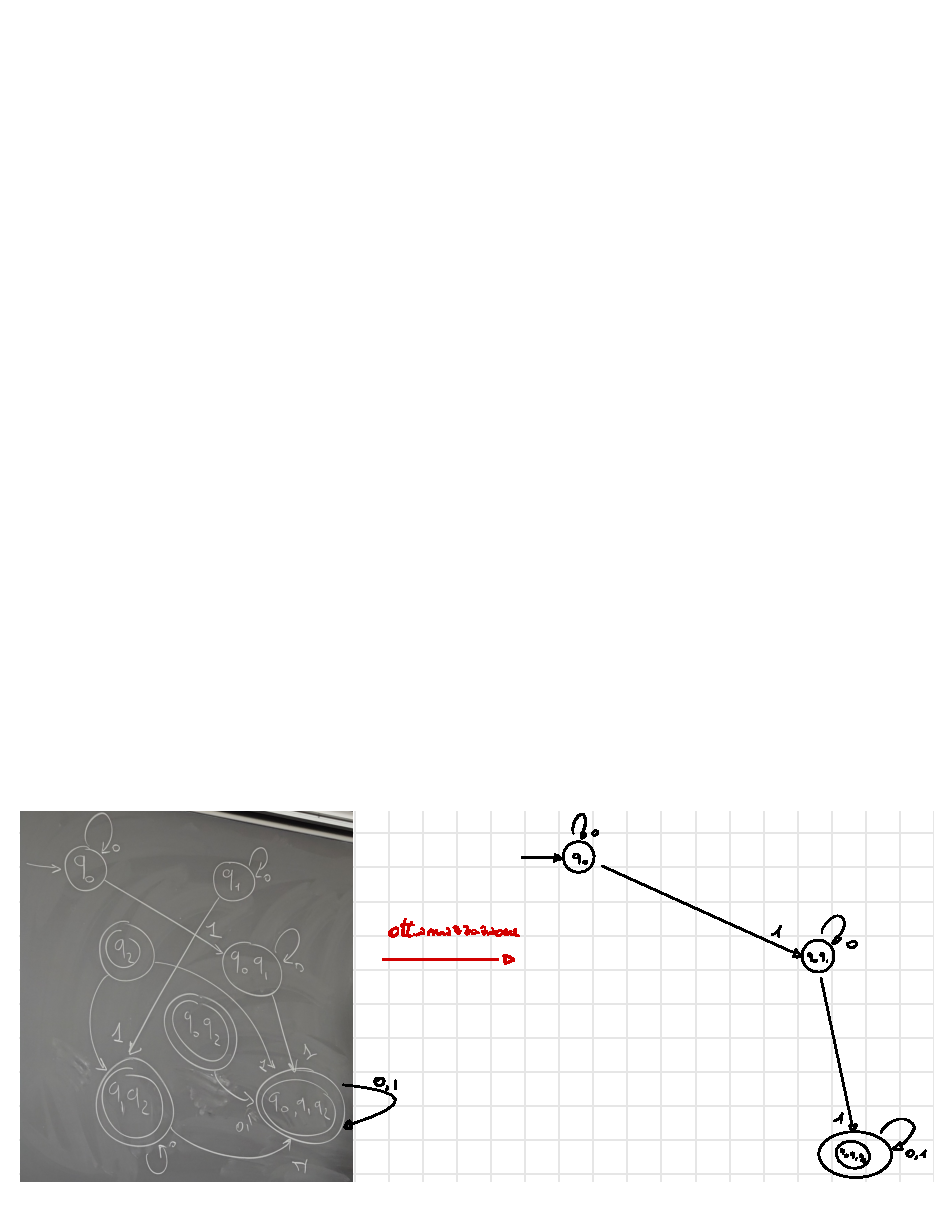
\includegraphics[width=1\textwidth]{img/grafo_ex2-sol.pdf}
		\caption{Rappresentazione di una conversione da non-deterministico a deterministico con relativa ottimizzazione.}
	\end{figure}
\end{document}